\documentclass[11pt]{article}

\setlength{\parindent}{0pt}
\usepackage{xltxtra}
\usepackage{hyperref}
\hypersetup{hidelinks}
\usepackage{url}
\urlstyle{tt}
\usepackage{xcolor}
\definecolor{CVBlue}{RGB}{23,110,191}
\usepackage{calc}
\usepackage{graphicx}
\usepackage{tikz}
\usetikzlibrary{calc}
\usepackage{fontspec}
\usepackage{xeCJK}
\usepackage{enumitem}
\CJKsetecglue{}

\setmainfont[
    Path = fonts/Main/,
    BoldFont = texgyretermes-bold.otf,
]{texgyretermes-regular.otf}

\setCJKmainfont[
    Path = fonts/hansans/,
    BoldFont = NotoSansSC-Bold.ttf,
]{NotoSansSC-Regular.ttf}

\usepackage{relsize}
\usepackage{xspace}
\usepackage{fontawesome}

\usepackage[
    a4paper,
    left=1.12cm,
    right=1.12cm,
    top=1.25cm,
    bottom=0.95cm,
    nohead
]{geometry}

\renewcommand{\baselinestretch}{1.17}

\usepackage{titlesec}
\setlist[itemize]{
    topsep=0.16em,
    itemsep=0.12em,
    parsep=0em,
    partopsep=0em,
    leftmargin=1.25em
}

\titleformat{\section}
{\large\bfseries\raggedright}
{}{0em}
{}
[{\color{CVBlue}\titlerule}]

\titlespacing*{\section}{0cm}{0.72em}{0.38em}

\newcommand{\cvsection}[2]{\section{#2}}

\newcommand{\datedentry}[3]{
    \textbf{#1} \hfill #2\\
    #3
}

\begin{document}
\pagenumbering{gobble}

% 头像
\begin{tikzpicture}[remember picture, overlay]
\node[anchor=north east] at ($(current page.north east)+(-1.2cm,-0.82cm)$)
{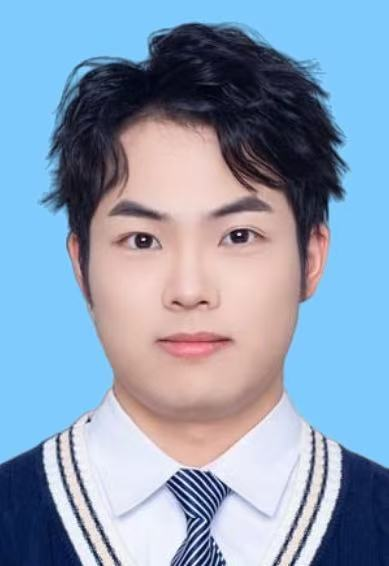
\includegraphics[height=2.35cm]{d57a13e6ad3a5b90a918a927d6181ced.jpg}};
\end{tikzpicture}

\centerline{\LARGE\bfseries{蒋豪}}
\vspace{0.06cm}
\centerline{\normalsize
\faEnvelopeO\ tinglanshen49@gmail.com \quad
\faPhone\ 15924302250 \quad
\faGithub\ \href{https://github.com/wealt2/ai_program}{github.com/wealt2/ai\_program}}

\vspace{0.08cm}

%%%%%%%%%%%%%%%%%%%%%%%%%%%%%%%%%%%%%%%%%%%%%%%%%%%%
\cvsection{\faUser}{个人简介}

中山大学天文学硕士在读，具备 Python 科学计算、机器学习建模、数据处理与可视化经验。曾围绕天琴卫星空间环境参数预测与非保守力分析构建神经网络模型，将电子数密度时间分辨率由 1 min 提升至 1 s；重视模型实验、结果复现与代码工程化沉淀。

%%%%%%%%%%%%%%%%%%%%%%%%%%%%%%%%%%%%%%%%%%%%%%%%%%%%
\cvsection{\faGraduationCap}{教育经历}

\datedentry{中山大学}{2024.09 -- 2027.07}{天文学（硕士）}

\vspace{0.08cm}
\datedentry{宁波工程学院}{2020.09 -- 2024.07}{材料成型及控制工程（学士）}

%%%%%%%%%%%%%%%%%%%%%%%%%%%%%%%%%%%%%%%%%%%%%%%%%%%%
\cvsection{\faUsers}{项目经历}

\textbf{天琴卫星所受太阳风动压与太阳光压分析} \hfill 科研项目
\begin{itemize}
    \item 面向天琴轨道周期内空间环境建模，利用机器学习预测不同时间点和位置对应的电子数密度、速度等参数，为动力学分析提供高分辨率输入。
    \item 基于神经网络构建时间序列回归模型，完成数据清洗、训练验证与误差分析，将电子数密度预测时间分辨率由 1 min 提升至 1 s；建立无拖曳控制模型分析非保守力影响。
\end{itemize}

\textbf{AI 语音绘图工具} \hfill \href{https://github.com/wealt2/ai_program}{github.com/wealt2/ai\_program}
\begin{itemize}
    \item 开发以语音为主要交互方式的二维绘图与 AI 图片创作 Web 应用；基础图形、尺寸、移动、旋转、撤销、保存等指令由本地规则解析器执行，复杂人物、场景与图片修改路由至 AI 服务。
    \item 使用原生 HTML/CSS/JavaScript 实现单页工作台，基于 Web Speech API、Speech Synthesis API 和原生 SVG DrawingEngine 支持中英文绘图指令、同义词/误识别容错、相对布局、尺寸继承、自转/公转、多对象旋转与执行步骤反馈。
    \item 设计本地矢量、AI DrawingPlan 与 AI 图片三类自动路由；通过 DeepSeek 扩写短语、追问关键词并生成绘图提示词，再交由 OpenAI/Gemini 进行图片生成、原位修改、局部蒙版和整体场景续绘。
    \item 采用 Cloudflare Pages + Worker 架构代理 AI 请求，将 API Key 保存在 Worker Secret，避免暴露到浏览器端；编写 Node.js 回归测试覆盖解析、绘图执行、AI 路由、图片对象、局部编辑和语音容错等场景，最近结果为 58/58 passed。
\end{itemize}

%%%%%%%%%%%%%%%%%%%%%%%%%%%%%%%%%%%%%%%%%%%%%%%%%%%%
\cvsection{\faCogs}{专业技能}

\textbf{编程与工程：} 熟练掌握 Python，常用 NumPy、Pandas、SciPy、Matplotlib 进行科学计算、数据清洗、特征处理与可视化；了解 Java 和 C++ 基础，能够阅读并理解代码逻辑。\\
\textbf{机器学习：} 熟悉监督学习与非监督学习，掌握 SVM、决策树、随机森林、K-Means、PCA 等方法，具备回归预测、聚类分析、模型评估与参数调优经验。\\
\textbf{深度学习：} 熟悉 FNN、CNN、RNN 的构建与训练流程，掌握 TensorFlow、PyTorch 等框架，了解 NLP 与 CV 基本方法。

%%%%%%%%%%%%%%%%%%%%%%%%%%%%%%%%%%%%%%%%%%%%%%%%%%%%
\cvsection{\faBook}{科研成果}

Li, C. F., Jiang, H., Su, W., et al.  
\textit{Methods and Results of the Study on Acceleration Noise due to Space Magnetic Field for Geocentric Orbit Gravitational Wave Detectors}.  
Astronomical Techniques and Instruments (Submitted), 2026.

%%%%%%%%%%%%%%%%%%%%%%%%%%%%%%%%%%%%%%%%%%%%%%%%%%%%
\cvsection{\faTrophy}{荣誉奖励}

\begin{itemize}
    \item 硕士研究生一等奖学金 \hfill 2024 -- 2025
    \item 硕士研究生三等奖学金 \hfill 2025 -- 2026
\end{itemize}

\end{document}
